\section{Redes Sociales} \label{sec:red}

La información contenida en la actual sección es tomada del libro \textit{Social Network Analisis for Startups} \cite{sna_startups}

\subsection{SNA: Social Network Analisis}

La administración de una red social fuera de línea fue estudiada desde inicios del siglo XX \cite{dynamics} con un enfoque socio-matemático llamado “análisis de redes sociales” (SNA por sus siglas en inglés: Social Network Analisis). Sin embargo, era difícil el análisis del comportamiento humano según los designios de la SNA, puesto que la información debía ser recopilada por medio de entrevistas a las personas. Aun así, el enfoque SNA fue utilizado para analizar el comportamiento terrorista o inclusive el comportamiento de trabajadores en una empresa. \cite{sna_startups}

\subsection{Analisis egocéntrico} \label{sec:egocentrico}

Los estudios basados en SNA pueden ser de tipo egocéntrico o sociocéntrico \cite{user_behavior}. En los estudios egocéntricos de una red social, se analiza un individual dentro de una red social y todas las conexiones de éste hacia otros individuales en la red social analizada. El individual analizado es llamado “ego” y los individuales que hacen conexión con él son llamados “alters”. Se han identificado 4 capas en el estudio de las redes egocéntricas, estas son:

\begin{itemize}
  \item Support clique: En esta capa se identifican los alters con los que el ego hace más contacto por alguna razón de peso para él (e.g. para obtener soporte emocional). Esta capa tiene, en promedio, 5 alters.
  \item Sympathy group: En promedio a éste corresponden 15 alters.
  \item Affinity group: En promedio a éste corresponden 50 alters.
  \item Active network: En promedio a éste corresponden 150 alters.
\end{itemize}

Los números dados en las capas descritas en el análisis egocéntrico son congruentes con el número de Dunbar, el cual representa el umbral promedio de número de alters sobre la capa “active network” (150) según Robin Dunbar, argumentando que este límite se debe a la capacidad cognitiva del cerebro humano \cite[Pag. 3]{dynamics} (como más adelante será nombrado, los servicios de redes sociales ayudan al ser humano a gestionar su active network, proporcionando herramientas que, en teoría y de acuerdo a la brecha tecnológica, lo ayudarán a mantener sus lazos con los alters de su red ego).

El análisis egocéntrico permite conocer los factores que dirigen al ego a crear vínculos débiles o fuertes con potenciales alters, albergándolos en alguna de las cuatro capas o en ninguna.

Con la creación de las OSN y la gran cantidad de información que describe el comportamiento humano sobre este tipo de red social, ha sido más sencillo utilizar el enfoque de la SNA para estudiar que comportamientos tienen los humanos sobre una red social establecida.

\subsection{Grado de centralidad}

En todas las redes, sean virtuales o no, existen personas que son mas ``importantes'' que otras, más \textbf{populares}. Estas celebridades representan una parte muy pequeña de la red, pero debido a su gran influencia siempre es bueno identificarlos. Para esto se utiliza el \textbf{grado de centralidad}.

El grado de un nodo es la cantidad de conexiones que posee. En una red social, esto se representa por medio de las relaciones que cada nodo tenga, y ya que el significado de la relación varía en función de cada red, es necesario entender que significan las posibles relaciones existentes en una red para hacer el análisis correspondiente. Por ejemplo, en una red como Twitter en donde las relaciones son unidireccionales, puede existir un nodo con un grado de salida muy alto, esto es una persona que sigue a muchas otras. Aunque esta persona tenga un grado de centralidad muy alto, no representa una celebridad, sin embargo, un nodo que tenga un grado de entrada muy alto, que es seguido por muchas personas, si representa una persona que es muy popular en esta red.

\begin{figure}[!htb]
  \begin{center}
    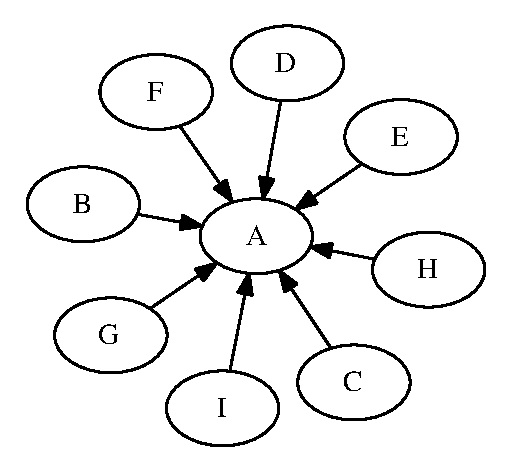
\includegraphics{./imagenes/red_estrella.eps}
    \caption{Red de estrella.}
    \label{fig:red_estrella}
    \textbf{Fuente:}  Autores
  \end{center}
\end{figure}


En la figura \ref{fig:red_estrella} se puede ver un caso en el que el nodo A es una clara celebridad de la red. Este tipo de configuración, llamada red de estrella, es muy poco común en la vida real, pero sirve de ayuda visual para entender a simple vista el concepto de centralidad.

\subsection{Grado de cercanía}

A menudo se puede ver que personas que no tienen mayor influencia aparente en una red son capaces de difundir un mensaje en una gran parte de la red. Esto se debe a que tienen buenas conexiones en la red que les permiten llegar a mas personas, sin que ellos en si sean ``importantes'' en la red. Para medir que tan bien o mal posicionado esta un nodo en la red se utiliza el \textbf{grado de cercanía}. Este calculo es bastante caro computacionalmente ya que conlleva una gran cantidad de cálculos.

Los pasos para calcular el grado de cercanía de los nodos de una red son:

\begin{enumerate}
  \item Calcular la ruta mas corta entre todos los pares de nodos posibles, utilizando el algoritmo de Dijkstra, y almacenar estos valores en una tabla.
  \item Para cada nodo de la red:
  \begin{enumerate}
    \item Calcular la distancia promedio con todos los demás nodos.
    \item Dividir el promedio por la distancia mas alta.
    \item Calcular el inverso del valor anterior.
  \end{enumerate}
  \item normalizar cada valor obtenido para obtener valores en el rango de 0-1.
\end{enumerate}

Los nodos que tengan un valor mas cercano a 1 son los que tienen una distancia promedio menor con los nodos de la red, o los que tienen ``\textit{mejores contactos}''.

\subsection{Factor distancia en la formación de las redes sociales}

La formación de redes sociales (tanto fuera de línea como en línea) es afecta por la distancia entre cada individual y el posible tipo de enlace que los uniría. En \cite{evolution} se hizo un estudio acerca de la formación de lazos, la formación de triadas entre individuales de una red social basada en la inscripción localizaciones recomendadas y frecuentadas por los usuarios, teniendo como parámetros ``la edad'' o tiempo de vinculación del individual a la red social, el grado de cada individual (número de conexiones que tiene un individual a otro) y la localización de cada individual en la red social. También se analizó cómo afectaba la creación de nuevos lazos con la movilidad del usuario (el desplazamiento por lugares geográficos distintos). En conclusión, se verificó que la formación de lazos depende proporcionalmente de la edad y del grado del individual y es inversamente proporcional a la distancia que a cada individual y que la formación de lazos puede modelarse con solo dos de los tres factores (el grado y la distancia); en cuanto a la formación de triadas, se verificó que ésta depende de las características sociales de la red, tomando énfasis en los individuales compartidos entre los posibles individuales formadores de triadas. Además, en cuanto a la creación de nuevos lazos teniendo en cuenta los lugares visitados por cada usuario de la red social, se presenta un patrón: Los usuarios escogen un lugar popular para visitar y, posteriormente, dirimen con que usuario crear un lazo teniendo en cuenta su popularidad y que frecuente los mismos lugares siempre.

\subsection{Grado de intermediación}

En las redes sociales, suelen formarse grupos mas pequeños que comparten un interés común. Por ejemplo, es mas probable que dos personas que comparten el gusto por los videojuegos interactúen entre si que dos personas que no lo hagan, sin embargo hay casos en los que una persona comparte gustos con diferentes grupos, ayudando a que esta persona se pueda relacionar de manera efectiva con un grupo mas extenso de personas. Estas personas son conocidas como ``puertas frontera'' ya que, gracias a ellos, es posible que dos grupos que no tengan nada en común puedan relacionarse entre sí. La medida que ayuda a identificar estos elementos en una red es el \textbf{grado de intermediación}, y consiste en lo siguiente:

\begin{enumerate}
  \item Calcular la ruta mas corta entre todos los pares de nodos posibles, utilizando el algoritmo de Dijkstra, y almacenar estos valores en una tabla.
  \item Para cada nodo n de la red, contar las veces que el nodo n aparece en la lista de rutas mas cortas,
  \item normalizar cada valor obtenido para obtener valores en el rango de 0-1.
\end{enumerate}

Cabe notar que este algoritmo es bastante lento para redes que son muy grandes.

En la figura \ref{fig:bow_tie} se puede ver un claro ejemplo de este fenómeno. Esta red, comúnmente denominada la "red corbatín" gracias a su forma similar a la de un corbatín, muestra como el nodo D se encuentra entre 2 grupos de nodos que, de otra manera, no podrían conectarse.

\begin{figure}[!htb]
  \begin{center}
    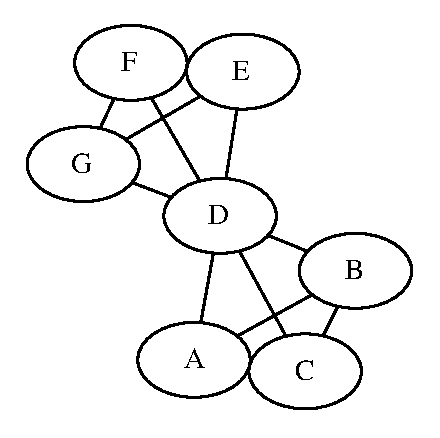
\includegraphics{./imagenes/bow_tie.eps}
    \caption{red corbatín.}
    \label{fig:bow_tie}
    \textbf{Fuente:}  Autores
  \end{center}
\end{figure}

\subsection{Díadas}

Las díadas son la unidad básica de análisis una red social, ya que estas representan la relación entre una y otra persona, esto es, mis amigos, mis seguidores, mis suscriptores, etc. Existen 4 tipos de díadas, representadas en la figura \ref{fig:tipos_diadas}, su uso varia en función del significado de la relación.

\begin{figure}[!htb]
  \begin{center}
      \begin{tabular}{m{3cm}|m{3cm}|m{3cm}|m{3cm}}
        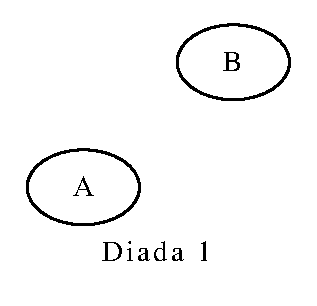
\includegraphics[width=3cm]{./imagenes/diada_1.eps} & 
        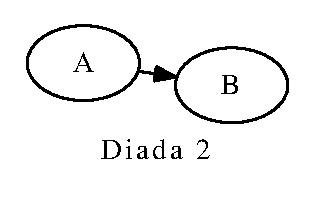
\includegraphics[width=3cm]{./imagenes/diada_2.eps} & 
        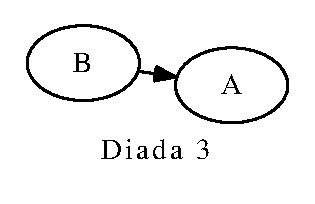
\includegraphics[width=3cm]{./imagenes/diada_3.eps} & 
        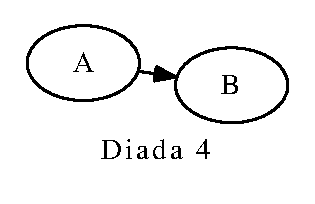
\includegraphics[width=3cm]{./imagenes/diada_4.eps}\\
      \end{tabular}
    \caption{Tipos de diadas asimétricas.}
    \label{fig:tipos_diadas}
    \textbf{Fuente:}  Autores
  \end{center}
\end{figure}


La díada 1 indica que ambos individuos existen en la red, pero todavía no existe ninguna relación entre ellos. Las diadas 2 y 3 muestran una relación unidireccional entre los dos individuos, la única diferencia es el sentido de esa relación. La díada 4, por su parte, es la de mayor interés de las cuatro ya que muestra una relación bidireccional entre los individuos, siendo esta la relación que mayor peso tiene en una red social dado que nos dice que existe un alto grado de reciprocidad en el intercambio de información entra ambos individuos.

\subsection{Tríadas}

Las triadas son básicamente 3 nodos conectados de alguna manera. Al igual que con las diadas, las triadas también pueden ser simétricas o asimétricas, dependiendo estrictamente del contexto en que son utilizadas. Existen 4 tipos de triadas simétricas, ilustradas en la figura \ref{fig:tipos_triadas_simetricas}.

\begin{figure}[!htb]
  \begin{center}
      \begin{tabular}{m{3cm}|m{3cm}|m{3cm}|m{3cm}}
        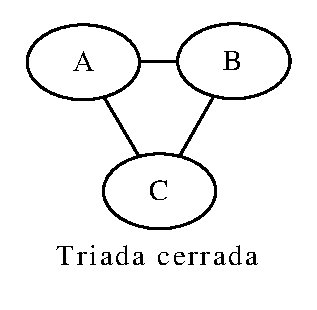
\includegraphics[width=3cm]{./imagenes/triada_simetrica_1.eps} & 
        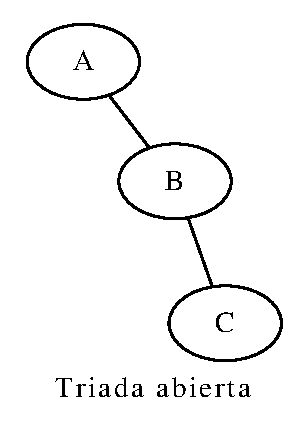
\includegraphics[width=3cm]{./imagenes/triada_simetrica_2.eps} & 
        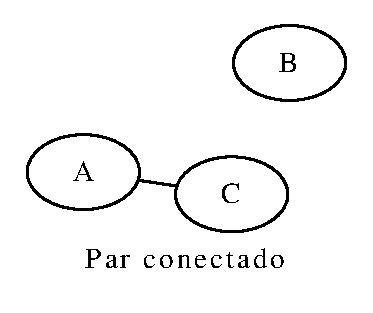
\includegraphics[width=3cm]{./imagenes/triada_simetrica_3.eps} & 
        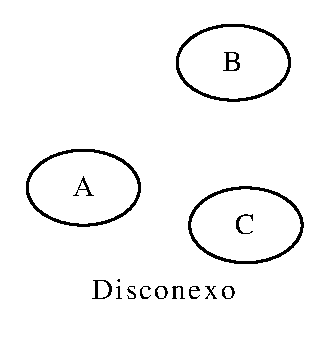
\includegraphics[width=3cm]{./imagenes/triada_simetrica_4.eps}\\
      \end{tabular}
    \caption{Tipos de triadas simétricas.}
    \label{fig:tipos_triadas_simetricas}
    \textbf{Fuente:}  Autores
  \end{center}
\end{figure}


Por otra parte, existen 16 tipos de triadas asimétricas, numeradas del 1-16. Su uso es mas frecuente ya que de ellas se puede hacer un análisis mas complejo en comparación a las díadas. Cada una de estas triadas recibe un nombre especifico para facilitar su identificación, a continuación se explica como debe leerse ese nombre:

\begin{itemize}
  \item El primer numero representa la cantidad de vértices bidireccionales
  \item El segundo numero representa la cantidad de vértices simples
  \item El tercer numero representa la cantidad de vértices inexistentes
  \item Si una triada se repite, se utiliza una letra extra para determinar que variante es:
  \begin{itemize}
    \item U - Arriba (Up)
    \item D - Abajo (Down)
    \item C - Circulo (Circle)
    \item T - Transitiva (Transitive)
  \end{itemize}
\end{itemize}

En la figura \ref{fig:tipos_triadas_asimetricas} se muestran todas las triadas posibles con su respectivo código asociado.

\begin{figure}[!htb]
  \begin{center}
      \begin{tabular}{m{1.3cm}|m{1.3cm}|m{1.3cm}|m{1.3cm}|m{1.3cm}|m{1.3cm}|m{1.3cm}|m{1.3cm}}
        \includegraphics[width=1.3cm]{./imagenes/triada_003.eps} & 
        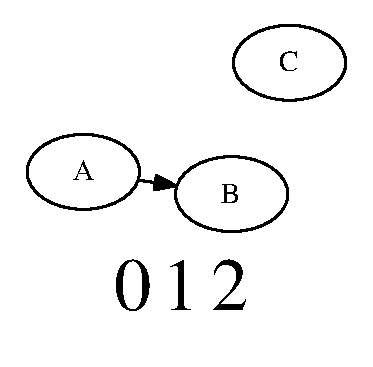
\includegraphics[width=1.3cm]{./imagenes/triada_012.eps} & 
        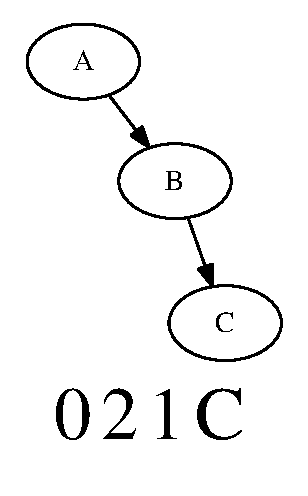
\includegraphics[width=1.3cm]{./imagenes/triada_021C.eps} & 
        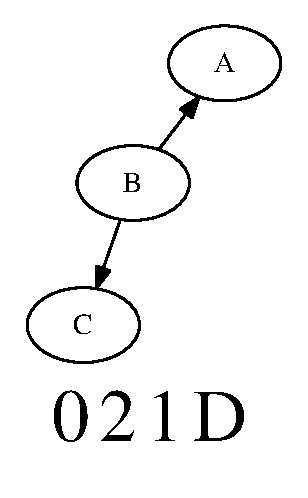
\includegraphics[width=1.3cm]{./imagenes/triada_021D.eps} & 
        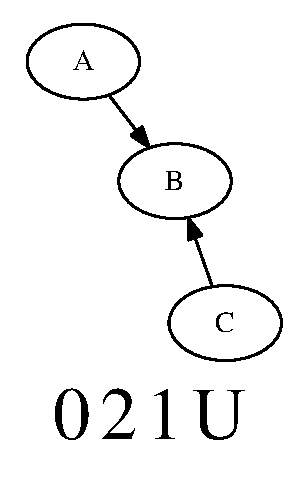
\includegraphics[width=1.3cm]{./imagenes/triada_021U.eps} & 
        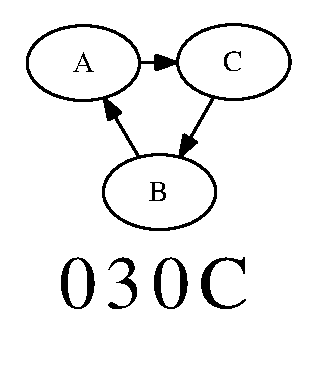
\includegraphics[width=1.3cm]{./imagenes/triada_030C.eps} & 
        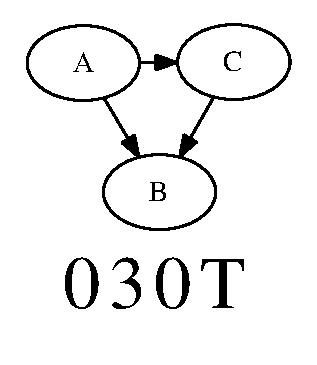
\includegraphics[width=1.3cm]{./imagenes/triada_030T.eps} & 
        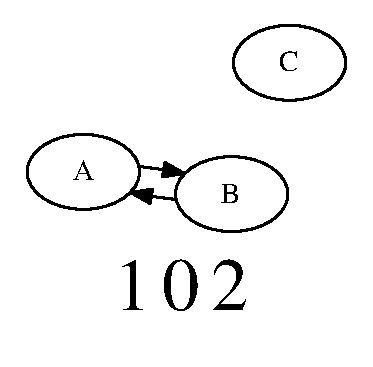
\includegraphics[width=1.3cm]{./imagenes/triada_102.eps}\\ \hline
        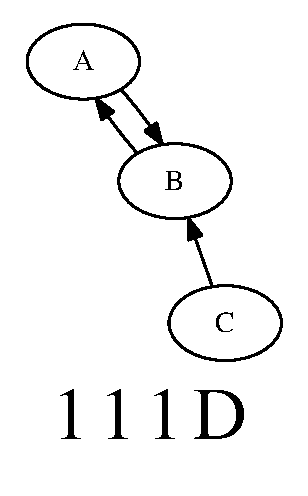
\includegraphics[width=1.3cm]{./imagenes/triada_111D.eps} & 
        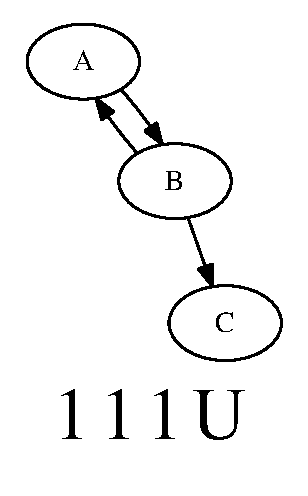
\includegraphics[width=1.3cm]{./imagenes/triada_111U.eps} & 
        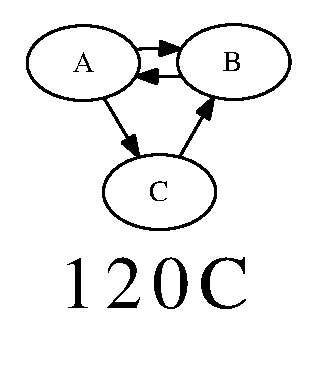
\includegraphics[width=1.3cm]{./imagenes/triada_120C.eps} & 
        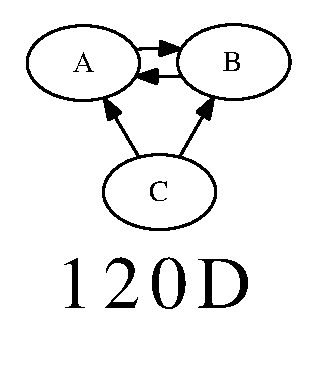
\includegraphics[width=1.3cm]{./imagenes/triada_120D.eps} & 
        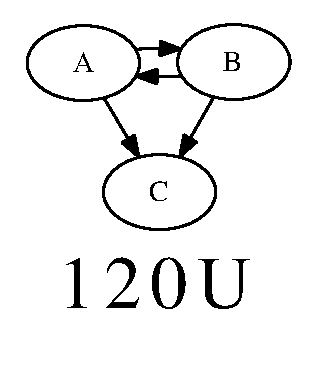
\includegraphics[width=1.3cm]{./imagenes/triada_120U.eps} & 
        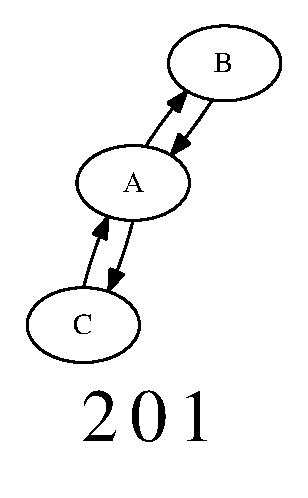
\includegraphics[width=1.3cm]{./imagenes/triada_201.eps} & 
        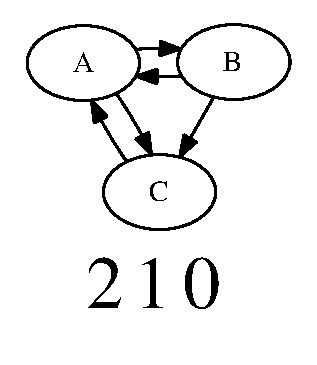
\includegraphics[width=1.3cm]{./imagenes/triada_210.eps} & 
        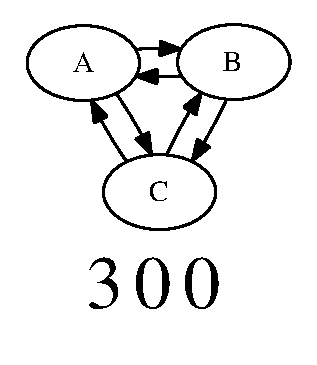
\includegraphics[width=1.3cm]{./imagenes/triada_300.eps}\\
      \end{tabular}
    \caption{Tipos de triadas asimétricas.}
    \label{fig:tipos_triadas_asimetricas}
    \textbf{Fuente:}  Autores
  \end{center}
\end{figure}


Gracias a esta discriminación topológica, se puede hacer un análisis mas completo de una red. Este análisis recibe el nombre de \textbf{\textit{Análisis Triadico}}.

\subsection{Análisis Triádico}

Este proceso, que también recibe el nombre de \textbf{Censo Triadico}, consiste en contar la ocurrencia de cada uno de los tipos de triada para cada nodo, y de esa forma determinar el rol que desempeña este nodo en la red. Por ejemplo, un nodo que presente en mayoría triadas del tipo 4, 7 y 11 es un nodo que \textbf{genera contenido}, mientras que si la mayoría de sus triadas son del tipo 5 y/o 10, es un nodo que recibe o \textbf{consume contenidos}.

Adicionalmente se puede hacer el mismo análisis a la red en general, para tener un punto de vista global de la red. En la figura \ref{fig:red_krackhardt} se puede ver una de las redes mas utilizadas en la teoría de redes sociales, la red de Krackhardt-kite. En esta red se pueden ver muchas características de una red social, facilitando el estudio de las mismas. Al hacer el censo a esta red, nos damos cuenta que presenta una gran cantidad de nodos tipo 201, que representan un agujero estructural, y nodos tipo 300, que representan triadas cerradas, esto nos indica que en esta red existen zonas que tienen una gran concentración de nodos interconectados, mientras hay zonas que no se encuentran muy pobladas. Todo esto se puede ver a simple vista en esta red, pero para redes mas grandes puede que represente un problema mayor.

\begin{figure}[!htb]
  \begin{center}
    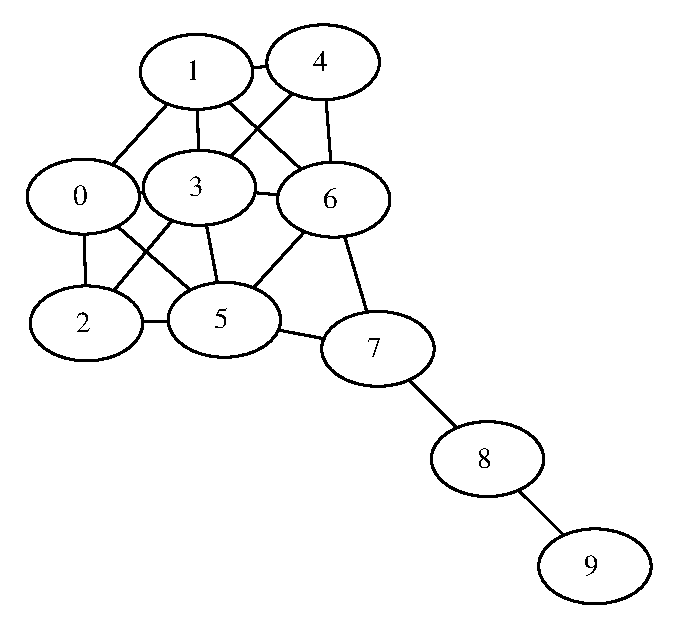
\includegraphics[width=8cm]{./imagenes/red_krackhardt_kite.eps}
    \caption{Red social de Krackhardt kite.}
    \label{fig:red_krackhardt}
    \textbf{Fuente:}  Autores
  \end{center}
\end{figure}



\section{UX - Análisis} \label{sec:UX}
Los servicios de redes sociales (SNS por sus siglas en ingles: Social Network Services) como Facebook, LinkedIn, Twitter, SportTracker o Xportia, ofrecen servicios para la gestión de la OSN de cada usuario que acceda a estas aplicaciones. Según un estudio hecho para medir la experiencia de usuario \cite{user_behavior_online} (UX por sus siglas en ingles: User eXperience) en los SNS, se encontraron 8 categorías que son críticas a la hora de diseñar una SNS y son:

\begin{enumerate}
  \item Self-expresion: Capacidad que tengan las OSN de compartir contenido relacionado a la vida real de los usuarios tal como lo pueden ser las fotos, los videos, los comentarios o las comunicaciones directas.
  \item Reciprocity: Interacción bilateral en tiempo real, es decir, interacción instantánea con uno o varios individuales en la OSN (por ejemplo, por medio de los servicios de mensajería instantánea).
  \item Learning: La información recibida por medio de la OSN debe poder ser utilizada en pro del desarrollo cognitivo del individual; debe existir información útil al individual que usa la OSN.
  \item Curiosity: El contenido de la OSN debe ser interesante para quien la utiliza.
  \item Suitability of functionality: Se refiere a cuán ``utilizable'' es una funcionalidad.
  \item Suitability of content: La calidad y exactitud de la información que en la OSN reside debe ser suficiente para el individual perteneciente a ella.
  \item Completeness of the user network: Los individuales deben querer pertenecer a la red social y buscar eficientemente a otros individuales para poder formar lazos con ellos y hacer crecer su red social.
  \item Trust and privacy: Confianza en los servicios de las OSN, así como también la capacidad que tiene el usuario de gestionar la privacidad del contenido que comparte en dicha OSN. \cite{social_experience}
\end{enumerate}

Cada uno de las categorías nombradas hace parte de los factores que impulsan la utilización de los SNS para la gestión de las OSN de las personas.
